\chapter{Top Physics}
\label{c:topPhys}


\section{Top quark physics history}
\fxnote{include ttbar and single}

\section{Four top quark production}

The production of four top quarks occurs predominantly via gluon fusion, as seen at leading order in Fig.~\ref{fig:ttttAtLO}~(left), with a $10\%$ contribution from quark-anti-quark annihilation. The production mechanism occurs via QCD whereas the decay of top quarks via W bosons is a weak interaction. 

\begin{figure}[ht!]
\begin{center}
    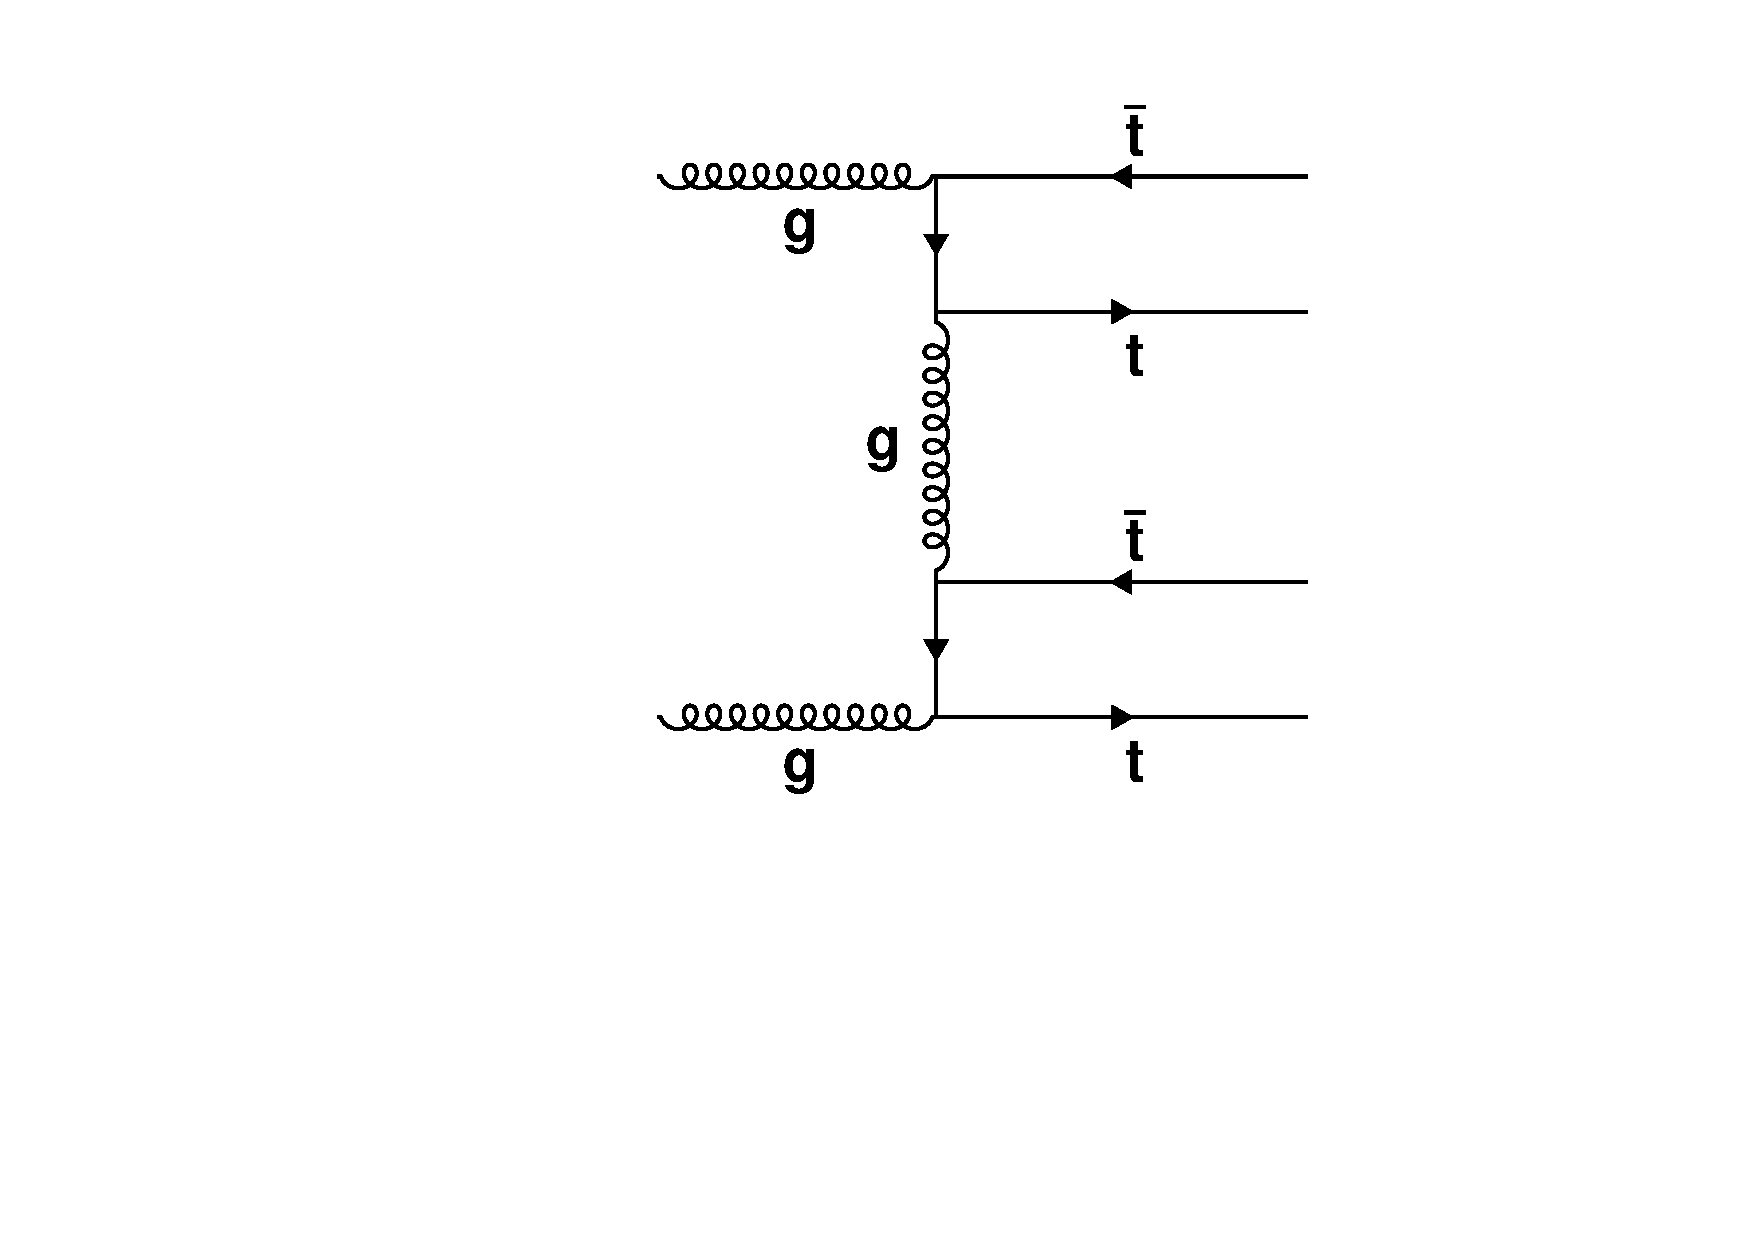
\includegraphics[width=0.49\textwidth]{images/Theory/tttt_t_LO.pdf}
    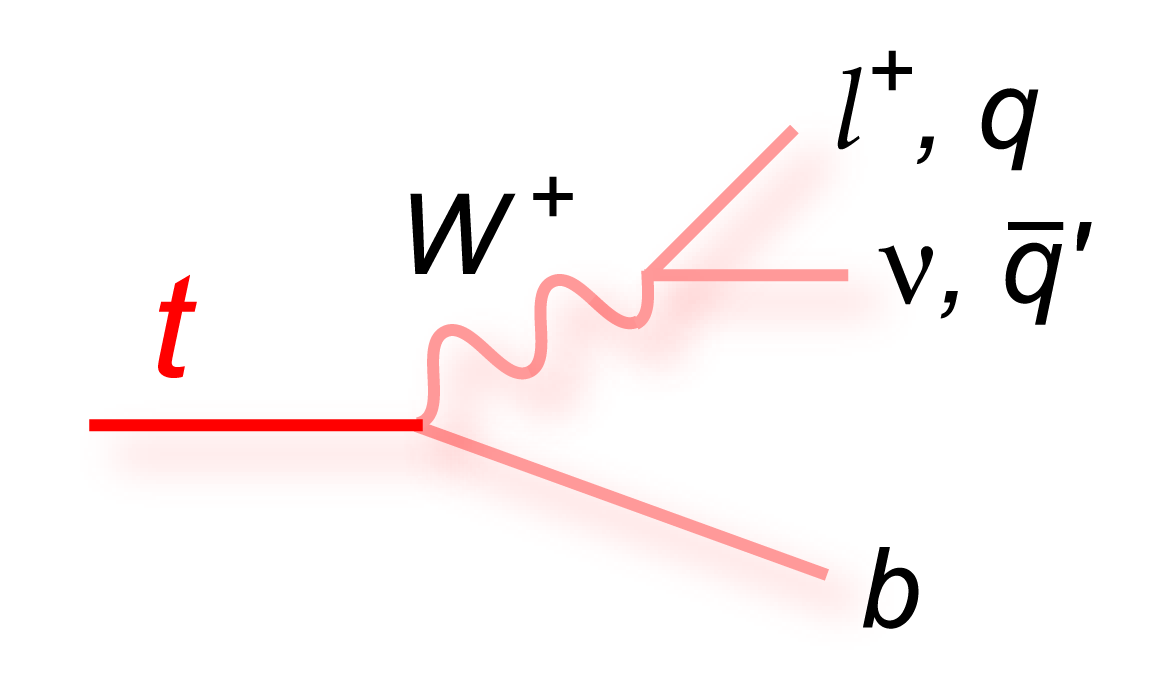
\includegraphics[width=0.49\textwidth]{images/Theory/topdecay.png}
    \caption{Dominant production mechanism for four top quarks in the standard model (left) an top quark decay to a W boson and b-quark with subsequent decay of the W boson either leptonically or hadronically (right).}
    \label{fig:ttttAtLO}
\end{center}
\end{figure}

Final states are determined by the decay of the W boson which can occur either leptonically or hadronically as seen in Fig.~\ref{fig:ttttAtLO}~(right). It can be seen from Fig.~\ref{fig:BRtttt} that the single lepton final state has the largest branching ratio which makes it a favourable place to look to study the largest number of events produced in the CMS detector. This is the final state considered most in this thesis. The dilepton final state also has a large branching ratio and has particularly low backgrounds when same-sign lepton final states are considered. The combination of studies on the dilepton final state will be discussed in Chapter~\ref{c:Run2}.

\begin{figure}[ht!]
\begin{center}
    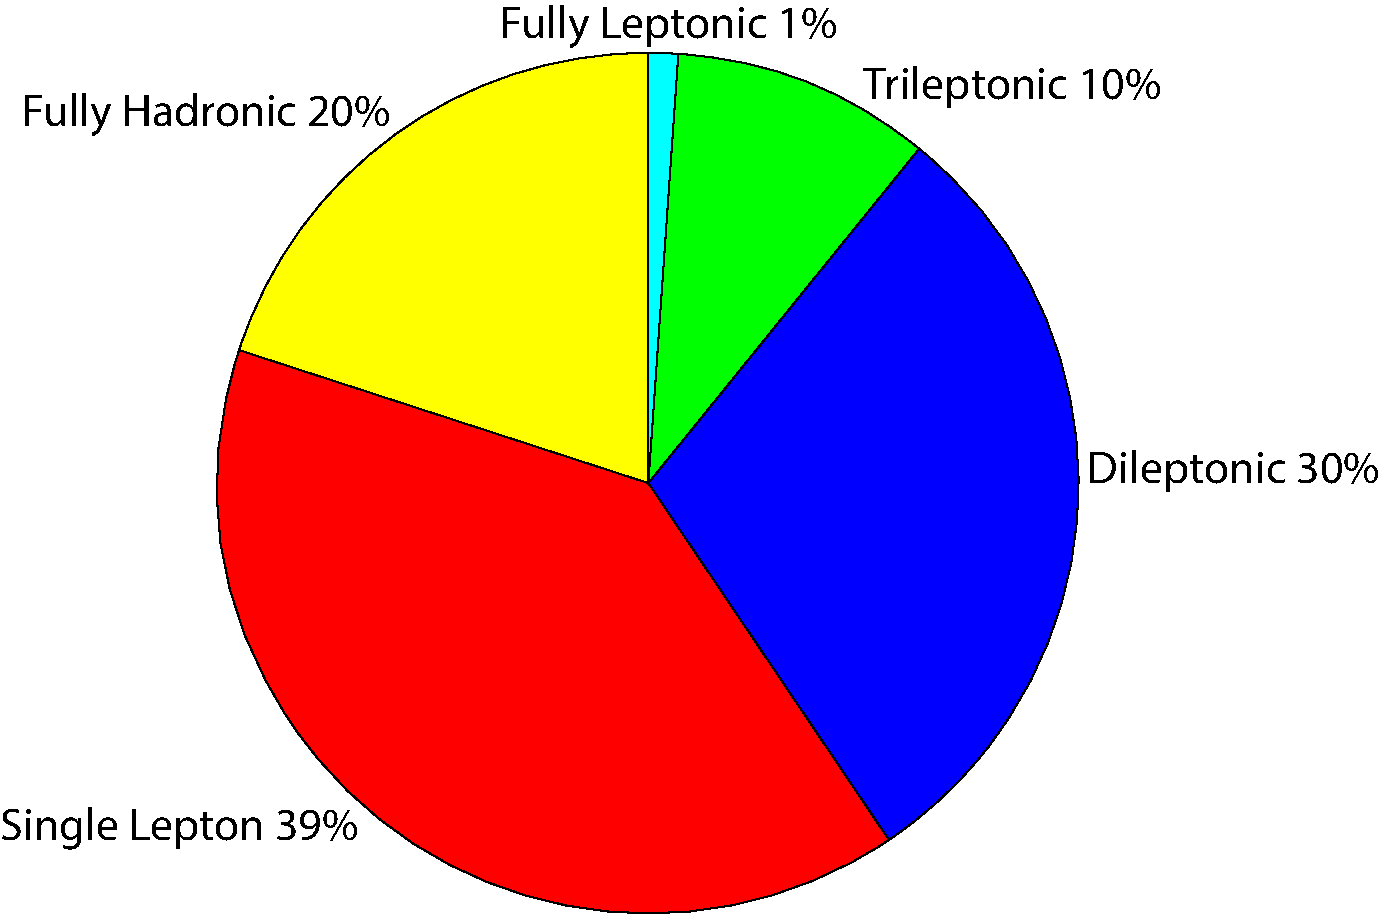
\includegraphics[width=0.4\textwidth]{images/Theory/FourTopBR.pdf}
    \caption{Branching ratios for final states as defined by leptonic decays.}
    \label{fig:BRtttt}
\end{center}
\end{figure}

